%!TEX program = xelatex
\documentclass[lang=cn]{elegantpaper}
\usepackage{listings}
\usepackage{xcolor}
\usepackage{threeparttable}
\usepackage{multirow}
\usepackage{CJK}
\usepackage{type1cm}
\usepackage{times}
\usepackage{bm}
\usepackage{float}
\usepackage[pdf]{graphviz}
\newcommand{\song}{\CJKfamily{song}}
\newcommand{\xiaoer}{\fontsize{18pt}{18pt}\selectfont}
\newcommand{\xiaosan}{\fontsize{15pt}{22pt}\selectfont}
\renewcommand{\baselinestretch}{1.8}    %两倍行距
\begin{document}

\section{逐步积分算法}
Opensees逐步积分算法共有12大类,包括AlphaOS($\alpha$ OS);BackwardEuler(Euler);
CentralDifference(CDM);
CollocationHS(CHS);GeneralizedAlpha(G-$\alpha$),HHT;Houbolt;KR-AlphaExplicit(KR-$\alpha$);Newmark;
ParkLMS3(PLMS3);
TRBDF;Wilson-Theta(W-$\theta$)法,如图\ref{tu1}所示。\\
其中:AlphaOS包括4种算法,如图\ref{tu2}所示,CDM包括3种算法,如图\ref{tu3}所示,HHT包括14种算法,如图\ref{tu4}所示,KR-AlphaExplicit算法包括2种算法,如图\ref{tu5}所示,,NEM算法类包括6种算法,如图\ref{tu6}所示。算法的具体介绍可见官网对\href{http://opensees.berkeley.edu/wiki/index.php/Integrator_Command}{Integrator}的解释及源代码。
\begin{figure}[H]		
	\centering
	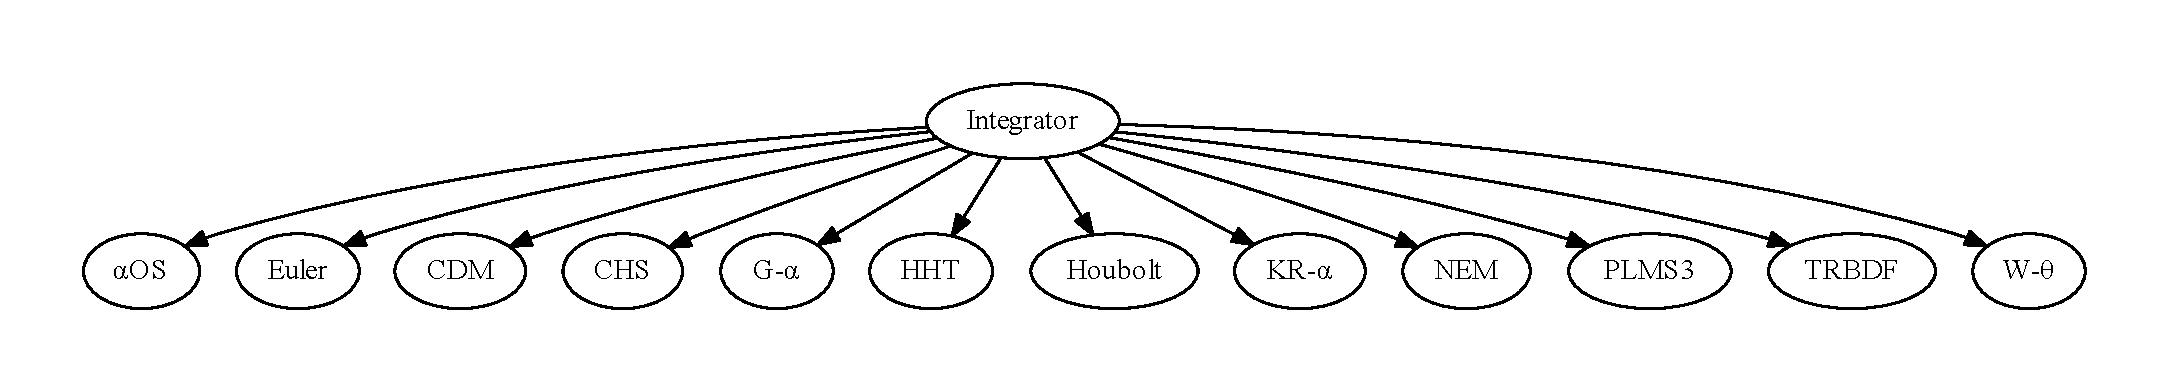
\includegraphics[width=1\textwidth]{Intergrator1.pdf}
	\caption{Opensees逐步积分算法}
	\label{tu1}
\end{figure}
\begin{figure}[H]		
	\centering
	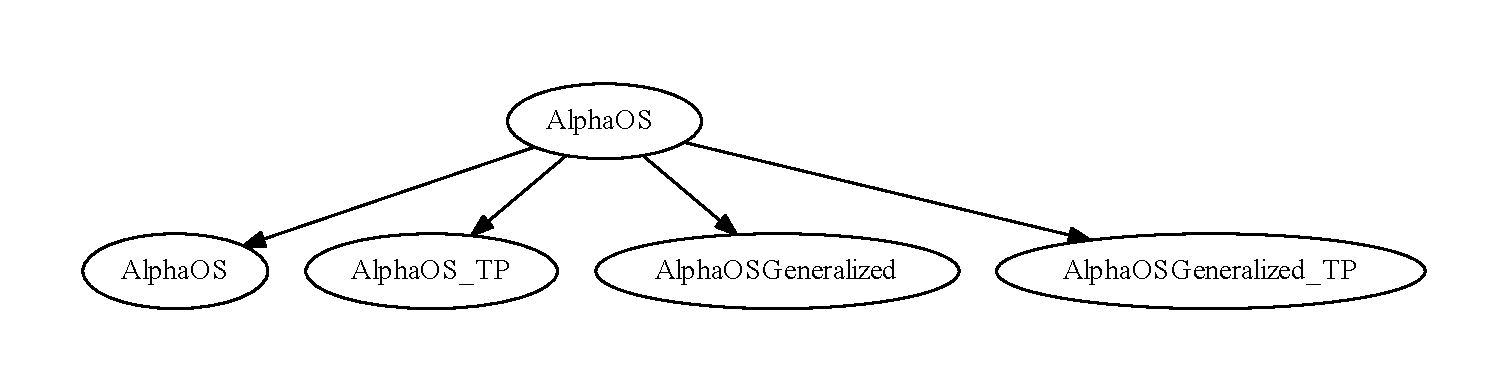
\includegraphics[width=0.8\textwidth]{AlphaOS.pdf}
	\caption{AlphaOS算法类}
	\label{tu2}
\end{figure}
%AlphaOS is an algorithmic class for performing a transient analysis using the Alpha-Operator-Splitting integration scheme. The parameter alpha corresponds to 1+alpha$\_${HHT}.\\
%\indent AlphaOSGeneralized$\_$TP is an algorithmic class for performing a transient analysisusing the generalized Alpha-Operator-Splitting integration scheme based on the trapezoidal rule. The parameters alpha correspond to 1+alpha$\_${HHT}.
\begin{figure}[H]		
	\centering
	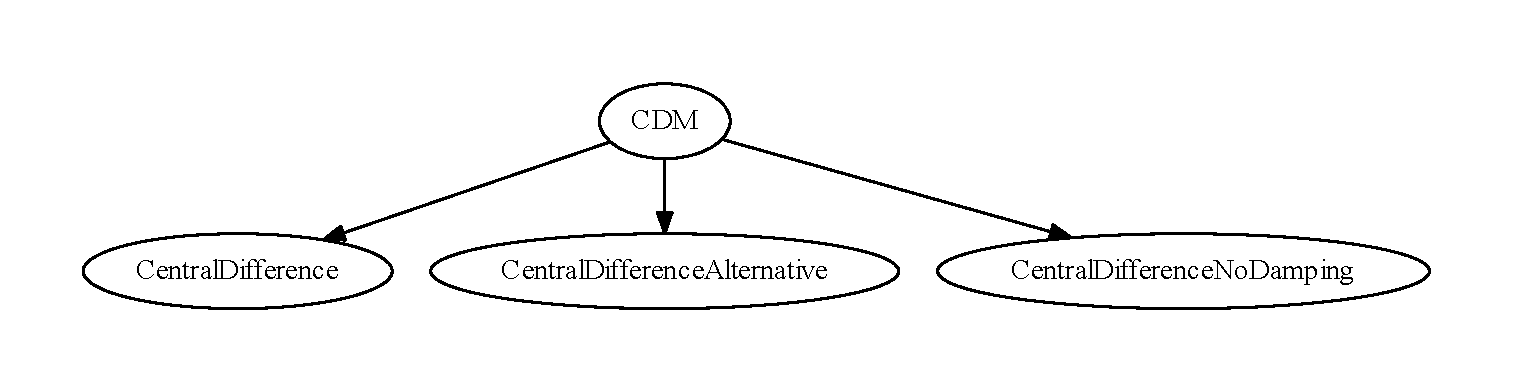
\includegraphics[width=1\textwidth]{CDM.pdf}
	\caption{CDM算法类}
	\label{tu3}
\end{figure}
\begin{figure}[H]		
	\centering
	 \begin{minipage}{1\textwidth}
	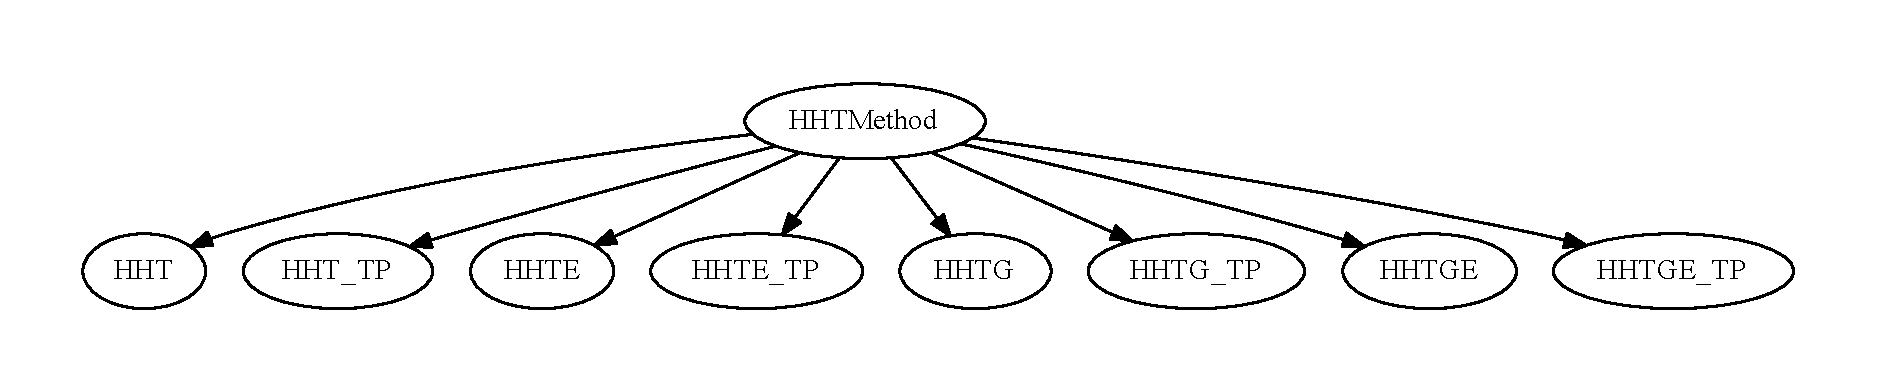
\includegraphics[width=1\textwidth]{HHT.pdf}
	\end{minipage}
	\begin{minipage}{1\textwidth}
		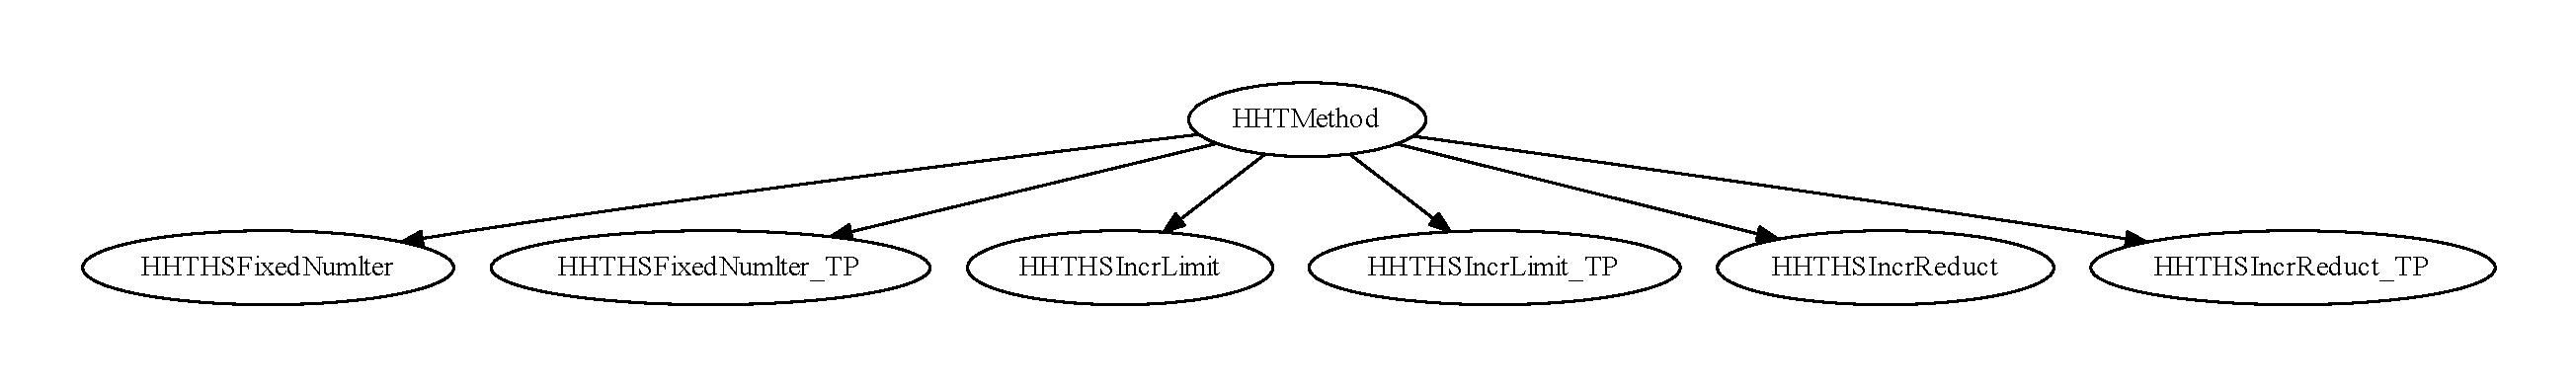
\includegraphics[width=1\textwidth]{HHT2.pdf}
	\end{minipage}			
	\caption{HHT算法类}
	\label{tu4}
\end{figure}
\begin{figure}[H]	
	\centering
	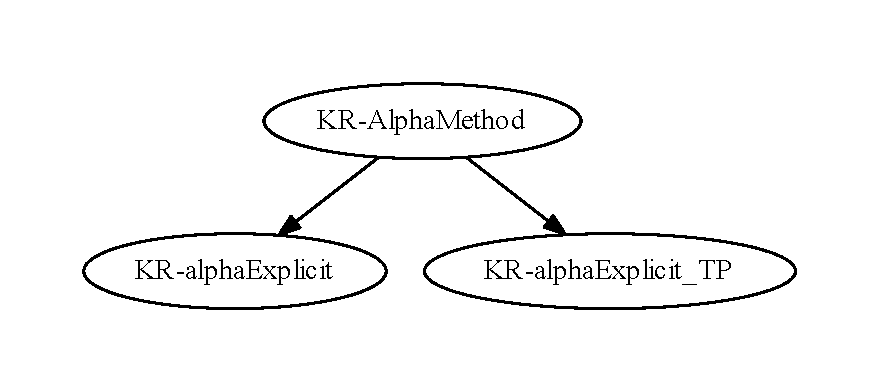
\includegraphics[width=0.7\textwidth]{KR.pdf}
	\caption{KR-AlphaExplicit算法类}
	\label{tu5}
\end{figure}	
\begin{figure}[H]		
	\centering
	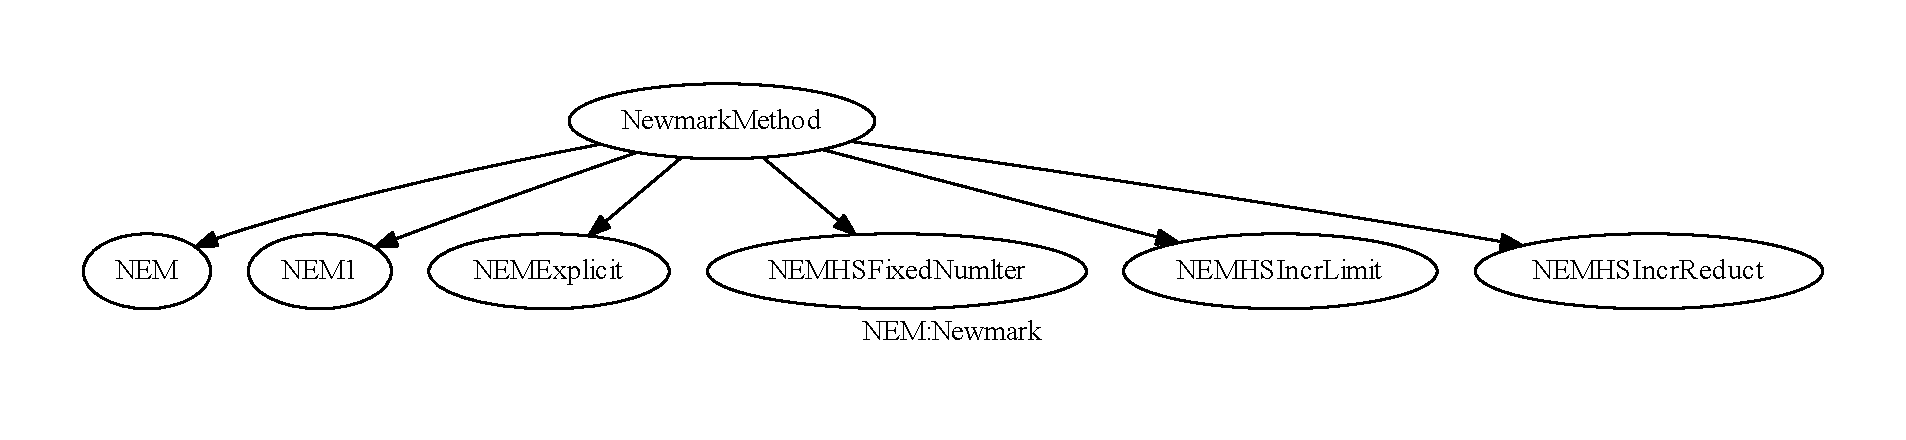
\includegraphics[width=1\textwidth]{NEM.pdf}
	\caption{NEM算法类}
	\label{tu6}
\end{figure}
\section{Element单元}

\begin{figure}[H]		
	\centering
	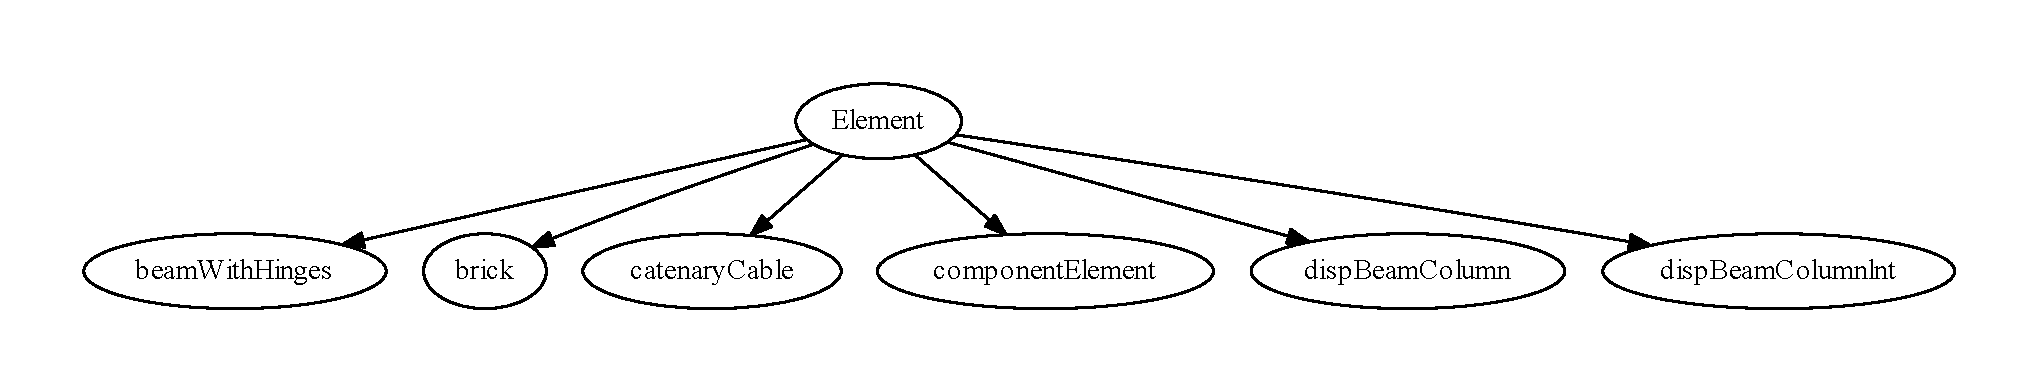
\includegraphics[width=1\textwidth]{Element1.pdf}
	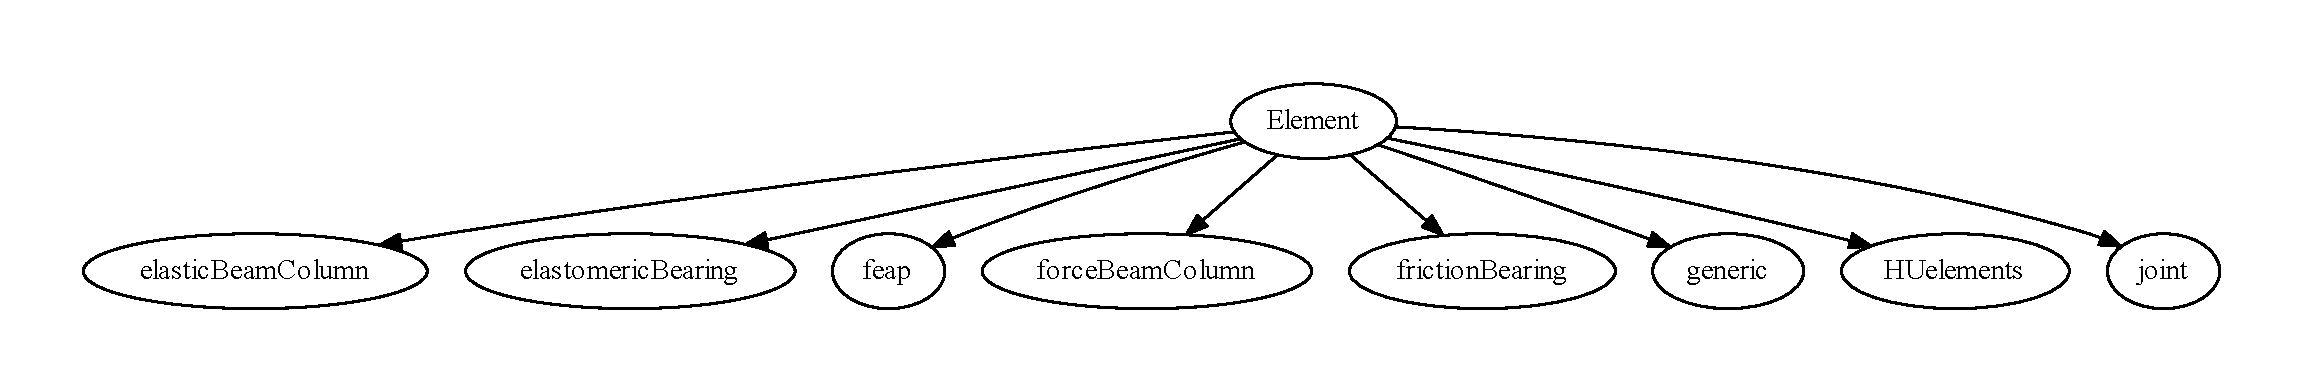
\includegraphics[width=1\textwidth]{Element2.pdf}
	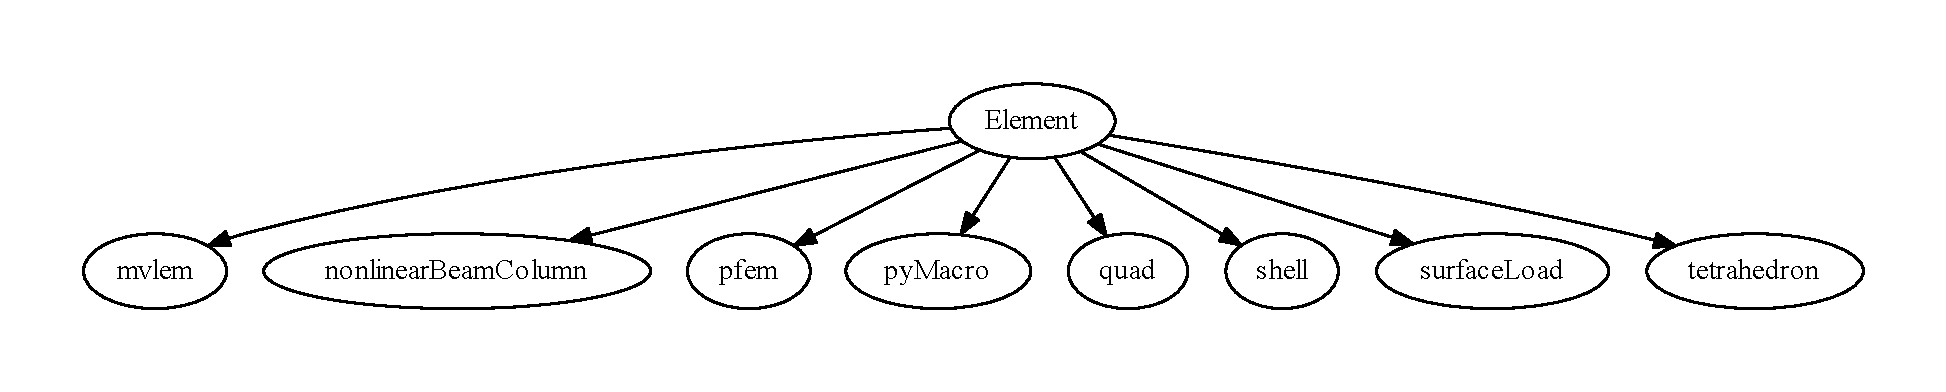
\includegraphics[width=1\textwidth]{Element3.pdf}
	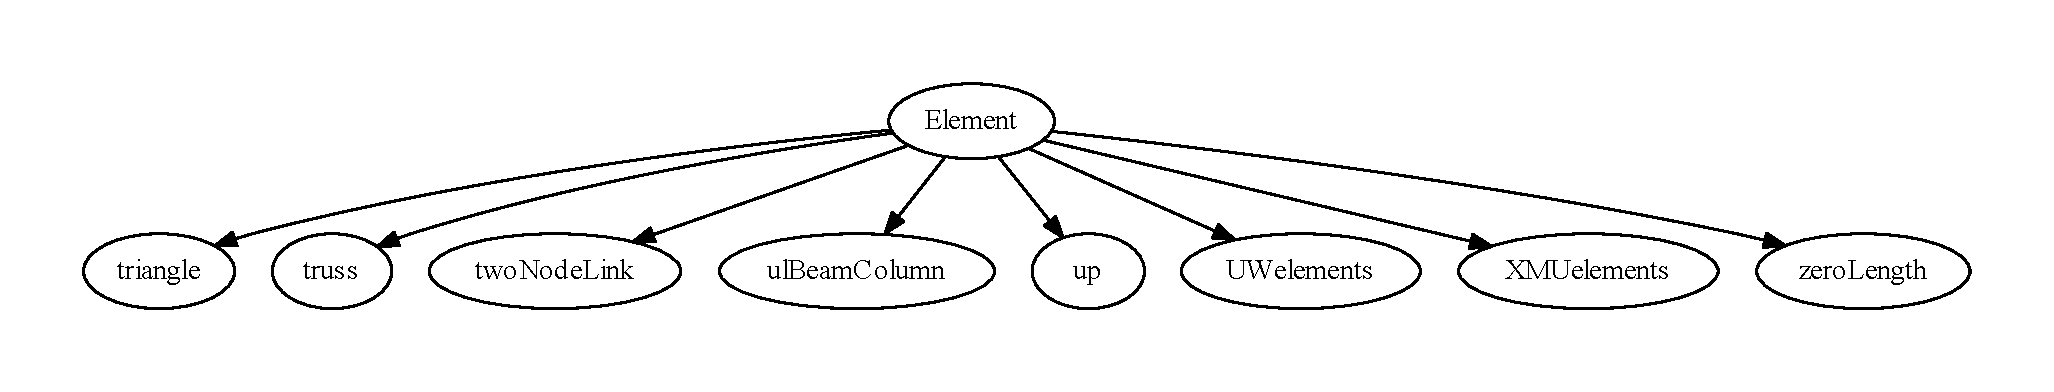
\includegraphics[width=1\textwidth]{Element4.pdf}
	\caption{Element分类}
	\label{tu7}
\end{figure}

\subsection{Truss Element} 
\subsubsection{Truss Element}
该命令用于构建一个桁架元素对象。 有两种方法来构建一个桁架元素对象:
一种方法是指定一个区域和一个UniaxialMaterial标识符:
\begin{lstlisting}
element truss $eleTag $iNode $jNode $A $matTag
\end{lstlisting}

\begin{figure}[H]		
	\centering
	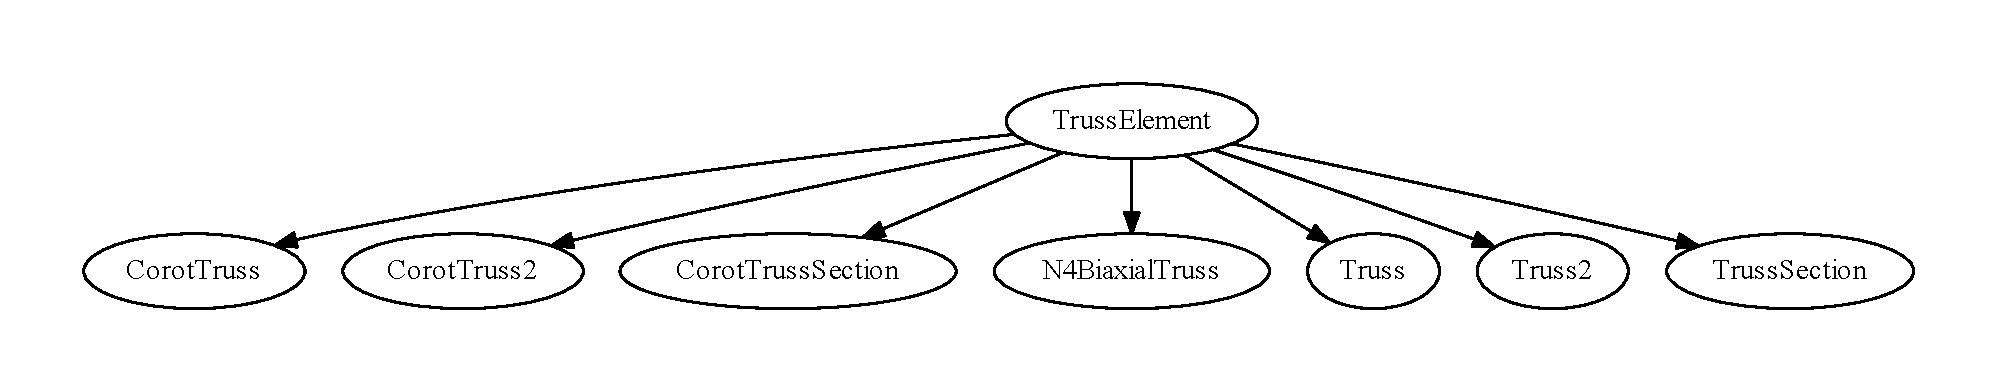
\includegraphics[width=1\textwidth]{Truss.pdf}
	\caption{Truss分类}
	\label{tu8}
\end{figure}

另一个是指定一个Section标识符:
\begin{lstlisting}
element truss $eleTag $iNode $jNode $secTag
	$eleTag - 独特的元素对象标签;
	$iNode $jNode - 端节点;
	$A - 元素的横截面积;
	$matTag - 与先前定义的UniaxialMaterial关联的标签;
	$secTag - 与先前定义的部分相关联的标签;
\end{lstlisting}
当用单轴材料构成时,桁架元件考虑应变率效应,因此适合用作阻尼元件。
当创建ElementRecorder对象时,对truss元素的有效查询是'axialForce','stiff',变形,'material matArg1 matArg2 ...','section sectArg1 sectArg2 ...'接口之后会有更多查询所涉及的方法。

\subsubsection{Corotational Truss Element}
该命令用于构建一个Corotational Truss(CorotTruss)元素对象。旋转公式采用一组随着元件旋转的旋转轴,从而考虑了局部和全局参照系之间的精确的几何变换。
有两种方法来构造一个Corotational Truss元素对象:
一种方法是指定一个区域和一个UniaxialMaterial标识符:
\begin{lstlisting}
element corotTruss $eleTag $iNode $jNode $A $matTag
\end{lstlisting}


另一个是指定一个Section标识符:
\begin{lstlisting}
element corotTruss $eleTag $iNode $jNode $secTag
$eleTag - 独特的元素对象标签;
$iNode $jNode - 端节点;
$A - 元素的横截面积;
$matTag - 与先前定义的UniaxialMaterial对象关联的标签;
$secTag - 与之前定义的Section对象关联的标记;
\end{lstlisting}



注意:当使用单轴材料对象构建时,桁架单元考虑应变率效应,因此适合用作阻尼单元。
当创建一个ElementRecorder对象时,对一个旋转桁架元素的有效查询是'axialForce','stiff','material $ matNum matArg1 matArg2 ...,''section $ secNum sectArg1 sectArg2 ...'
\subsection{Elastic Beam Column Element}
该命令用于构造一个elasticBeamColumn元素对象。 构造弹性梁柱单元的论据取决于问题的维数ndm:
对于一个二维问题:
\begin{lstlisting}
element elasticBeamColumn $eleTag $iNode $jNode $A $E $Iz $transfTag
\end{lstlisting}
对于一个三维问题:
\begin{lstlisting}
element elasticBeamColumn $eleTag $iNode $jNode $A $E $G $J $Iy $Iz $transfTag
\end{lstlisting}
创建ElementRecorder时对弹性梁柱元素的有效查询是'stiffness'和'force '。
\begin{figure}[H]		
	\centering
	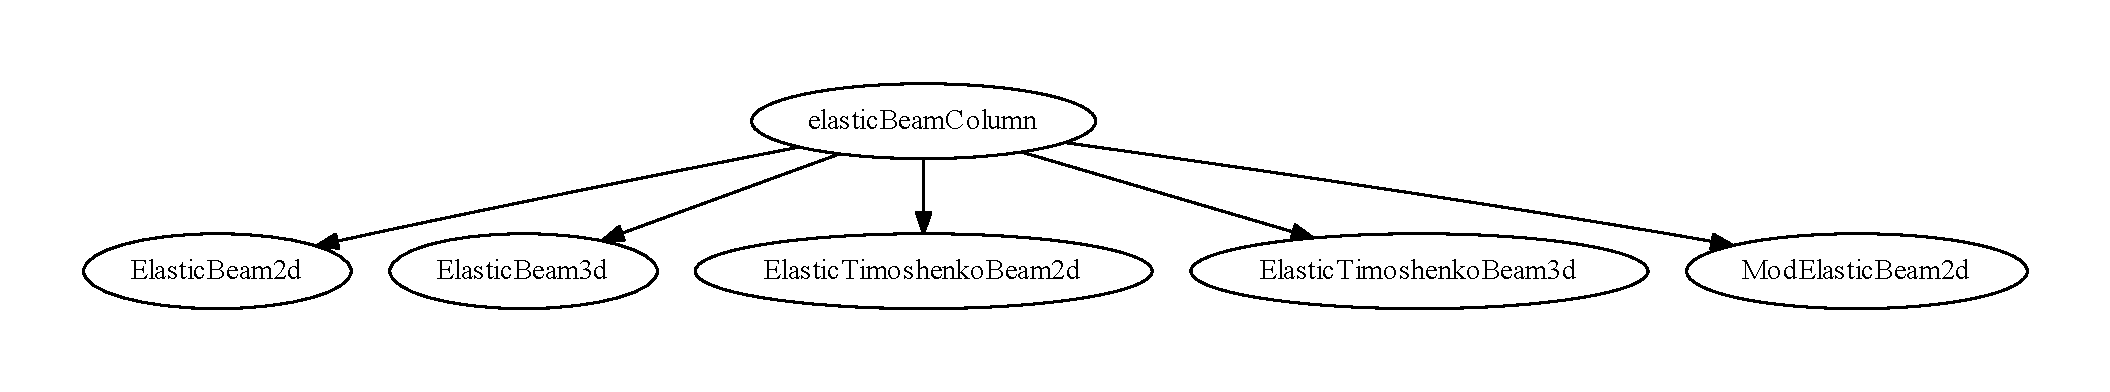
\includegraphics[width=1\textwidth]{elasticBeamColumn.pdf}
	\caption{elasticBeamColumn分类}
	\label{tu9}
\end{figure}





\subsection{NonLinear Beam-Column Elements}
有两种基本类型的非线性梁柱单元:
\begin{enumerate}
	\item 基于力的单元:分布可塑性(NonlinearBeamColumn),内部具有弹性的可塑性(beamwithHinges)
	\item 基于位移的单元:线性曲率分布的分布可塑性(dispBeamColumn)
\end{enumerate}
\begin{figure}[H]		
	\centering
	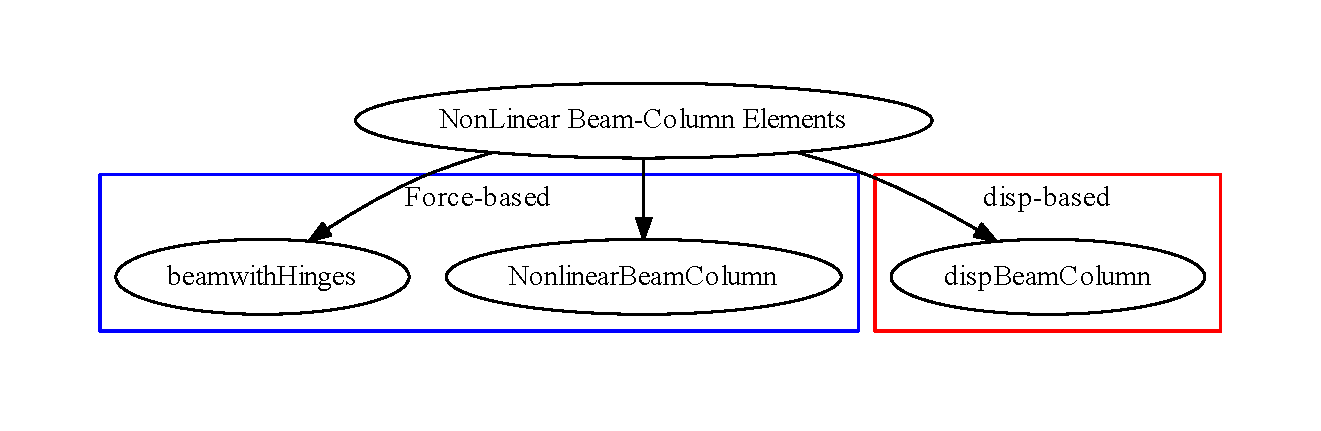
\includegraphics[width=1\textwidth]{NonlinearBeamColumn.pdf}
	\caption{Nonlinear Beam-Column分类}
	\label{tu10}
\end{figure}

\begin{lstlisting}
element nonlinearBeamColumn $eleTag $iNode $jNode $numIntgrPts $secTag $transfTag <-mass $massDens> <-iter $maxIters $tol>
\end{lstlisting}


这个命令用来构造一个非线性的BeamColumn元素对象,它是基于非迭代(或迭代)力的公式,并且考虑到沿着元素的可塑性扩展

对于一个二维问题:
\begin{lstlisting}
element beamWithHinges $eleTag $iNode $jNode $secTagI $Lpi $secTagJ $Lpj $E $A $Iz $transfTag <-mass $massDens> <-iter $maxIters $tol>
\end{lstlisting}


对于一个三维问题:
\begin{lstlisting}
element beamWithHinges $eleTag $iNode $jNode $secTagI $Lpi $secTagJ $Lpj $E $A $Iz $Iy $G $J $transfTag <-mass $massDens> <-iter $maxIters $tol>
\end{lstlisting}

这个命令被用来构造一个beam With Hinges元素对象,它是基于非迭代的(或迭代的)灵活性公式,并且认为可塑性集中在元素末端的指定铰链长度上。\\
请注意,beamHithges元素只在元素端定位塑性铰。\\
这种类型的元素将元素分为三个部分:两个端部的铰链和中间的线性元素区域。铰链是通过分配给每个以前定义的部分来定义的。每个铰链的长度也由用户指定。
\begin{lstlisting}
element dispBeamColumn $eleTag $iNode $jNode $numIntgrPts $secTag $transfTag <-mass $massDens>
\end{lstlisting}
此命令用于构造一个dispBeamColumn元素对象,它是一个分布式可塑性,基于位移的梁柱元素。
\subsection{ZeroLength Elements}
%ZeroLength Elements包括:Zero-Length Elements,Zero-Length ND Element,Zero-Length Section Element.
\begin{figure}[H]		
	\centering
	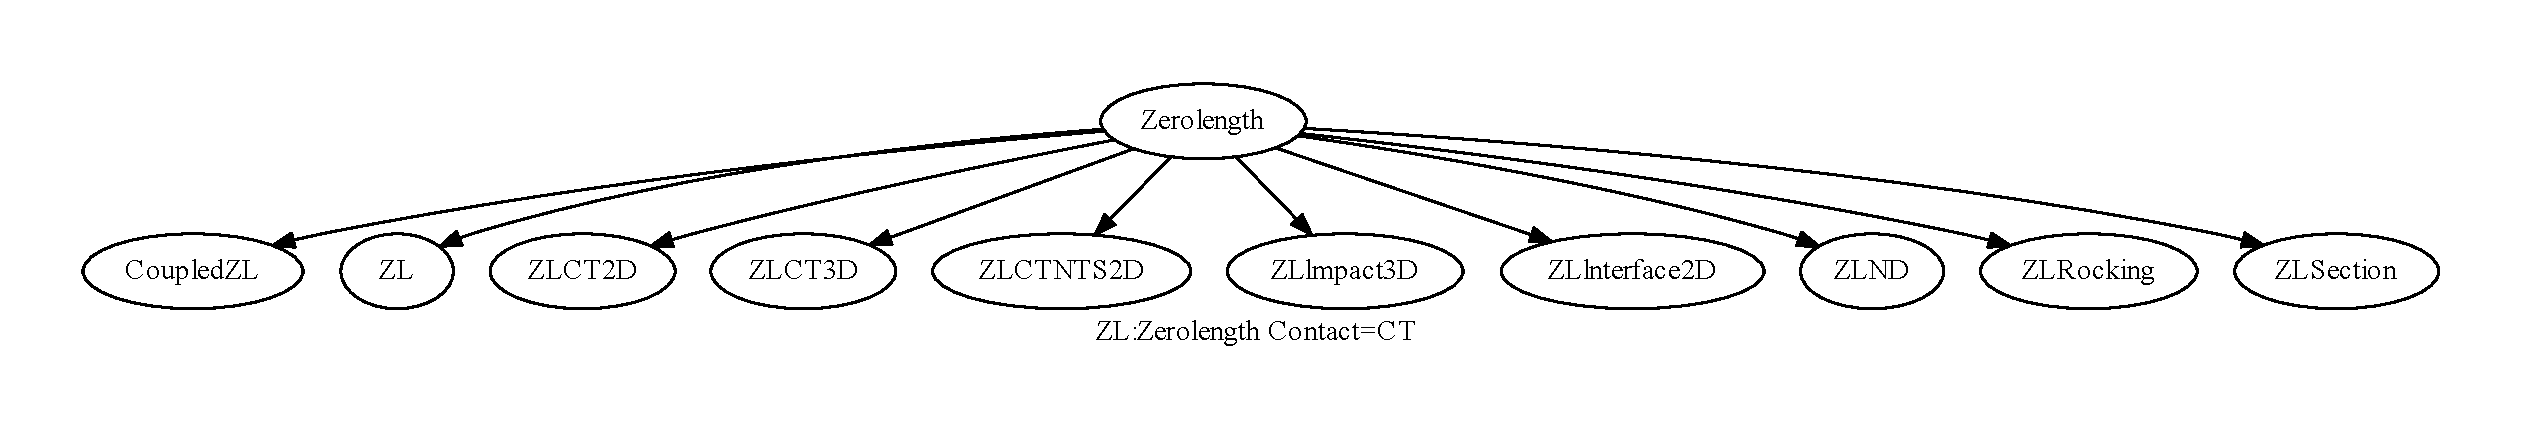
\includegraphics[width=1\textwidth]{ZeroLength.pdf}
	\caption{ZeroLength Elements分类}
	\label{tu11}
\end{figure}

\subsection{quad Element}
\begin{figure}[H]		
	\centering
	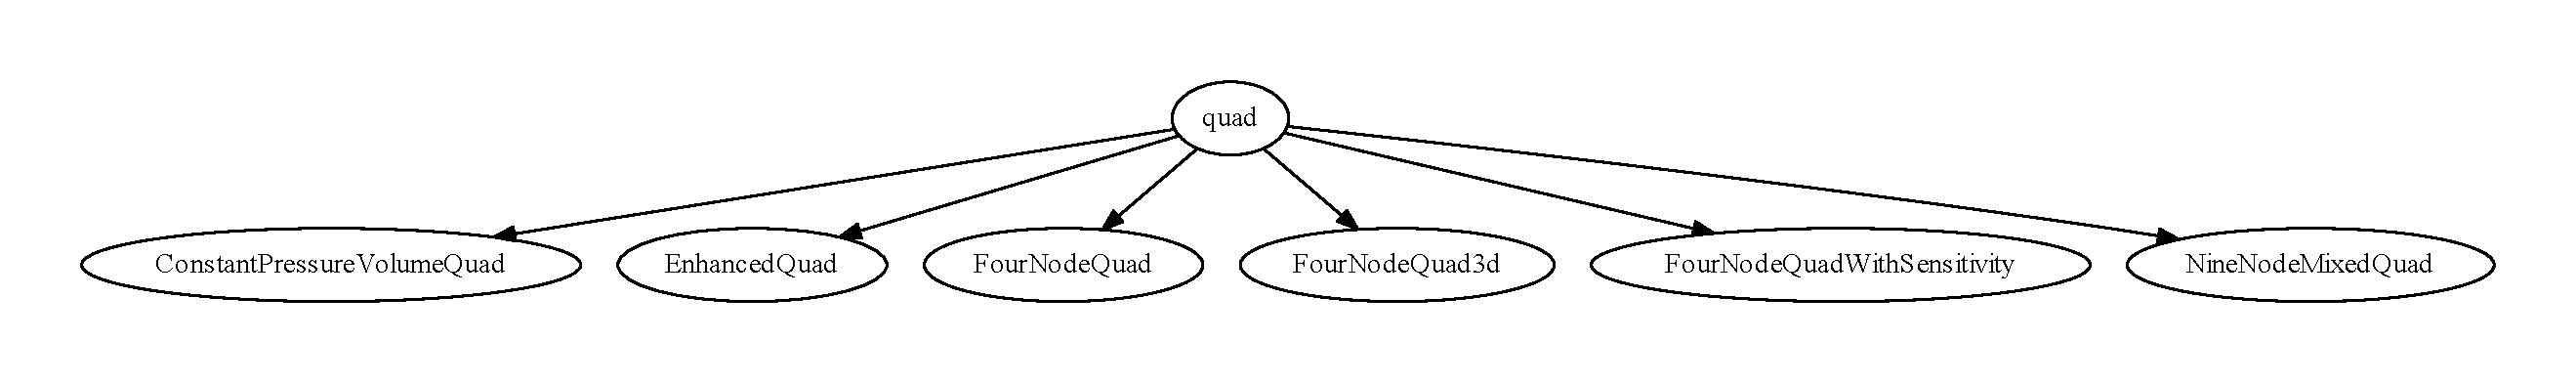
\includegraphics[width=1\textwidth]{quad.pdf}
	\caption{quad Elements分类}
	\label{tu12}
\end{figure}
\subsection{ Shell Element}
\begin{figure}[H]		
	\centering
	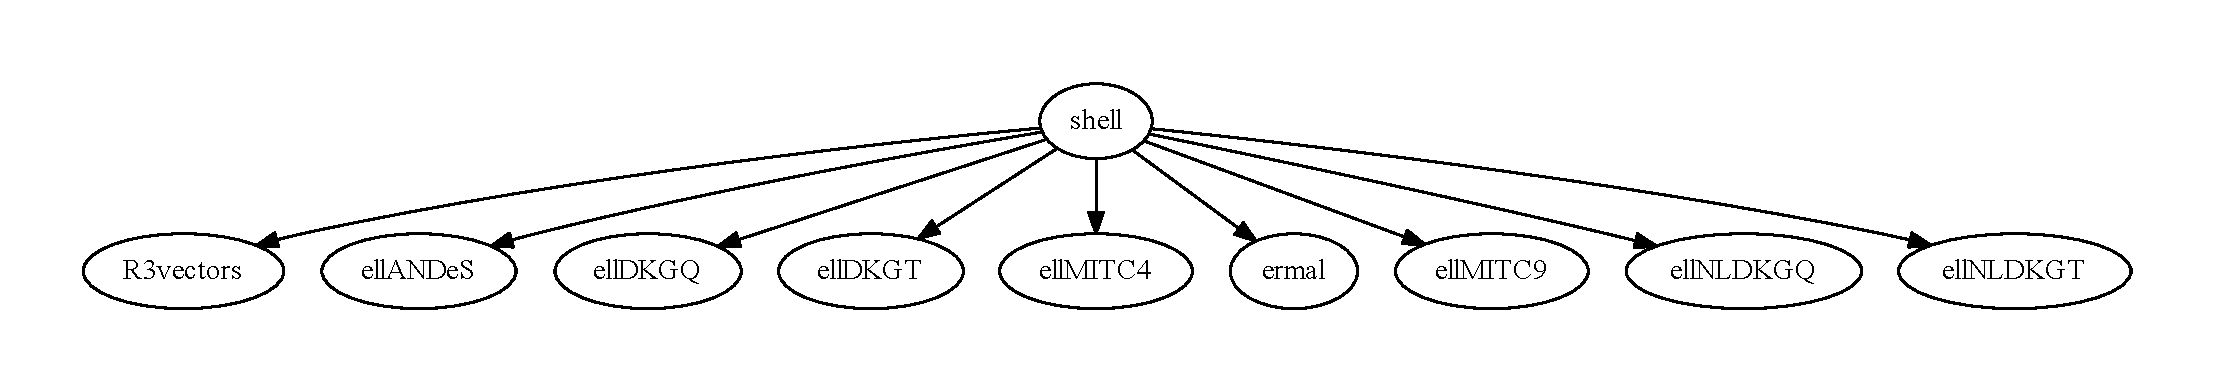
\includegraphics[width=1\textwidth]{shell.pdf}
	\caption{shell Elements分类}
	\label{tu12}
\end{figure}
\subsection{brick Element}
\begin{figure}[H]		
	\centering
	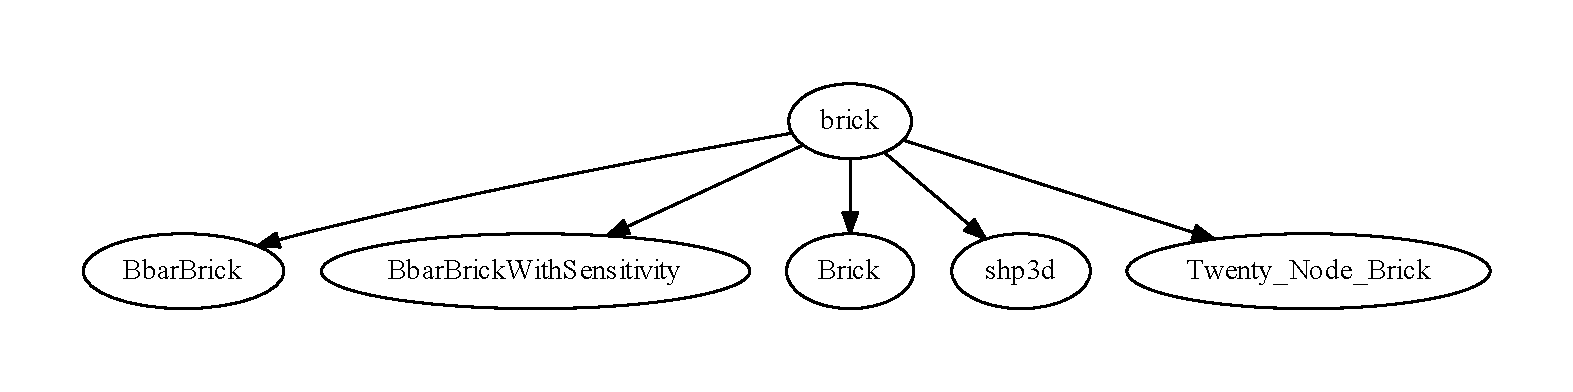
\includegraphics[width=1\textwidth]{brick.pdf}
	\caption{brick Elements分类}
	\label{tu12}
\end{figure}


















\end{document}
